\begin{frame}
 \frametitle{Outline}
 \tableofcontents
\end{frame}

\section{Fundamentals \\ \normalsize \textcolor{black!60!bgcolorAlt}{Algebras, Modules, Quivers}}

\begin{frame}{Algebras}
 \begin{alertblock}{$k$-algebra}
 	An algebra over a field $k$ is a $k$-vector space equipped with a
 	\alert{bilinear product}.
 \end{alertblock}
 \pause
 \textbf{Motivating examples}
 \begin{itemize}
  \item Complex numbers as the vector space $\R^2$ with the typical product of
   complex numbers.
  \pause
 	\item Ring of polynomials (over $k$) with polynomial multiplication.
 	\pause
 	\item Ring of square matrices with matrix multiplication.
 \end{itemize}
\end{frame}

\begin{frame}{Modules}
 \begin{alertblock}{$\Lambda$-module}
  Let $\Lambda$ be a $k$-algebra. A right $\Lambda$-module is a pair $(M, \cdot
  )$ where $M$ is a $k$-vector space and $ \cdot :M \times A \to M$ is a binary
  operation satisfying natural commutativity and associativity rules.
 \end{alertblock}
 \pause
 \textbf{Examples}
 \begin{itemize}
  \item Each algebra is a module (left or right) over itself.
  \pause 
 	 \item $k[x,y] = (k[x])[y]$ is a module (left or right) over $k[x]$.
 \end{itemize}
 \pause
 \begin{block}{Indecomposability (`prime' modules)}
 	A (right) $\Lambda$-module $M$ is \alert{indecomposable} if $M \neq 0$ and $M
 	= M_1 \oplus M_2$ implies that $M_1 = 0$ or $M_2 = 0$.
 \end{block}
\end{frame}

\begin{frame}{Module homomorphisms}
 \begin{alertblock}{$\Lambda$-module homomorphism}
 	A map $f:M \to N$ between two (right) $\Lambda$-modules $M$ and $N$ is a
 	$\Lambda$-module homomorphism if it's $k$-linear and respects $ \cdot $, that
 	is
 	\[
 	 f(m \cdot \lambda) = f(m) \cdot \lambda \text{ for } \lambda \in \Lambda, m
 	 \in M.
 	\]
 \end{alertblock}
 \pause
 \begin{block}{Section/retraction}
 	A $\Lambda$-module homomorphism $f:M \to N$ is
 	\vspace*{-\parskip}
 	\begin{itemize}
 	 \item a \alert{section} if $ \exists g: N \to M$ such that $g \circ f = 1_N$.
 	 \item a \alert{retraction} if $ \exists h: N \to M$ such that $f \circ h =
 	 	1_M$.
 	\end{itemize}
 \end{block}
\end{frame}

\begin{frame}[fragile]
 \frametitle{Module homomorphisms}
 \begin{block}{Irreducibility (`prime' homomorphisms)}
 	A $\Lambda$-module homomorphism $f:M \to N$ is \alert{irreducible} if
 	\begin{itemize}
 	 \item $f$ is neither a \textbf{section} nor a \textbf{retraction};
 	 \pause
 	 \item whenever $f = f_2 \circ f_1$, then $f_2$ is a retraction or $f_1$ is a
 	 	section.
 	\end{itemize}
 	We denote the $k$-vector space of irreducible homomorphisms $M \to N$ as
 	$\mathrm{Irr}(M,N)$.
 \end{block}
 \begin{figure}[h]
  \centering
  \begin{tikzcd}
   M \ar[rr, "f"] \ar[dr, "f_1"'] & & N \\
   															 & X \ar[ur, "f_2"'] &
  \end{tikzcd}
 \end{figure}
\end{frame}

\begin{frame}[fragile]
 \frametitle{Quivers}
 \begin{alertblock}{Quiver}
 	A \alert{quiver} is an oriented graph with multiple edges and loops.
 \end{alertblock}
 \pause
 \textbf{Examples}
 \begin{figure}[h]
  \centering
 	\begin{subfigure}[c]{.49\textwidth}
 	 \centering
	 \tikzset{every loop/.style={min distance=5mm,looseness=20}}
 	 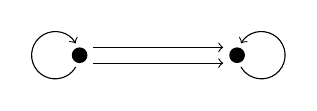
\begin{tikzpicture}
		\node[circle,fill,inner sep=2pt] (a) at (0,0) {};
		\node[circle,fill,inner sep=2pt] (b) at (2,0) {};
		\draw[->,shorten <=5pt,shorten >=5pt] (0, 0.1) -- (2, 0.1);
		\draw[->,shorten <=5pt,shorten >=5pt] (0, -0.1) -- (2, -0.1);
		\draw[<-] (-0.05,0.15) arc (30:330:0.3);
		\draw[<-] (2.05,0.15) arc (150:-150:0.3);
 	 \end{tikzpicture}
  \end{subfigure}
  \pause
 	\begin{subfigure}[c]{.49\textwidth}
 	 \centering
 	 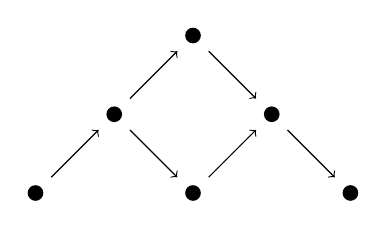
\begin{tikzpicture}
 	 	\node[circle,fill,inner sep=2pt] (a) at (0,0) {};
 	 	\node[circle,fill,inner sep=2pt] (b) at (1,1) {};
 	 	\node[circle,fill,inner sep=2pt] (c) at (2,0) {};
 	 	\node[circle,fill,inner sep=2pt] (d) at (2,2) {};
 	 	\node[circle,fill,inner sep=2pt] (e) at (3,1) {};
 	 	\node[circle,fill,inner sep=2pt] (f) at (4,0) {};

 	 	\draw[->,shorten <=5pt, shorten >=5pt] (a) -- (b);
 	 	\draw[->,shorten <=5pt, shorten >=5pt] (b) -- (c);
 	 	\draw[->,shorten <=5pt, shorten >=5pt] (b) -- (d);
 	 	\draw[->,shorten <=5pt, shorten >=5pt] (c) -- (e);
 	 	\draw[->,shorten <=5pt, shorten >=5pt] (d) -- (e);
 	 	\draw[->,shorten <=5pt, shorten >=5pt] (e) -- (f);
 	 \end{tikzpicture}
  \end{subfigure}
 \end{figure}
\end{frame}

\section{Auslander-Reiten Theory \\ \normalsize
\textcolor{black!60!bgcolorAlt}{Path Algebras, Representations, AR Quivers}}

\begin{frame}[fragile]
 \frametitle{Path algebras}
 \begin{alertblock}{The path algebra of a quiver}
  Let $Q$ be a quiver. The \alert{path algebra} $kQ$ of $Q$ is the $k$-algebra
  whose $k$-vector space has as its basis all paths of length $ \geq 0$ in $Q$
  and the product of two basis elements is the concatenation of paths.
 \end{alertblock}
\end{frame}

\begin{frame}[fragile]
 \frametitle{Path algebras -- Example}
 Consider the quiver
 \begin{figure}[h]
  \centering
  \begin{tikzpicture}
   \node[circle,fill,inner sep=2pt] (a) at (0,0) {};
   \node[circle,fill,inner sep=2pt] (b) at (2,0) {};
   \node[below=1mm of a] {$1$};
   \node[below=1mm of b] {$2$};
   \draw[->, shorten <=5pt, shorten >=5pt] (b) to node[above] {$a$} (a);
  \end{tikzpicture}
 \end{figure}

 \pause
 The basis of the path algebra $kQ$ is the triple $(e_1,e_2,a)$ (where $e_i$
 means `stay at $i$') and its multiplication table is
 \begin{table}[h]
  \centering
  \begin{tabular}{c|ccc}
   & $e_1$ & $e_2$ & $a$ \\
   \toprule
   $e_1$ & $e_1$ & $0$ & $0$\\
   $e_2$ & $0$ & $e_2$ & $a$\\
   $a$ & $a$ & $0$ & $0$
  \end{tabular}
 \end{table}

 \pause

 It's actually isomorphic to the $k$-algebra of lower triangular $2 \times 2$
 matrices over $k$.
\end{frame}

\begin{frame}
 \frametitle{Every algebra is a path algebra}
 \begin{theorem}
 	Let $k$ be an algebraically closed field and $\Lambda$ a basic, connected and
 	finite-dimensional algebra over $k$. Then there exists a finite connected
 	quiver $Q$ such that $\Lambda = kQ / I$ for some admissible ideal $I$ of $kQ$.
 \end{theorem}
 \pause
 \begin{theorem}
 	Let $\Lambda$ be as above. Then, $\Lambda = kQ$ for a quiver $Q$ if and only
 	if $\Lambda$ is \alert{hereditary} (submodules of projective modules are
 	projective).
 \end{theorem}
\end{frame}

\begin{frame}
 \frametitle{Dynkin quivers}
 \begin{theorem}[Gabriel's]
 	Let $\Lambda$ be as above. Then, $\Lambda = kQ$ where $Q$ (as an indirected
 	graph) is \alert{Dynkin} if and only if $\Lambda$ is
 	\alert{representation-finite} (the number, up to isomorphism, of
 	indecomposable finite-dimensional $\Lambda$-modules is finite).
 \end{theorem}
\end{frame}

\begin{frame}
 \frametitle{Dynkin quivers}
 \begin{figure}[h]
  \centering
  \begin{tikzpicture}
   \node[circle,fill,inner sep=2pt] (a) at (0,0) {};
   \node[circle,fill,inner sep=2pt] (b) at (1,0) {};
   \node[circle,fill,inner sep=2pt] (c) at (2,0) {};
   \node at (3,0) {$\cdots$};
   \node[circle,fill,inner sep=2pt] (d) at (4,0) {};
   \node[left=3mm of a] {$A_n:$};

   \draw (a) -- (b);
   \draw (b) -- (c);
   \draw (c) -- (2.5,0);
   \draw (3.5,0) -- (d);
	 
	 \begin{scope}[yshift=-1.5cm]
  	\node[circle,fill,inner sep=2pt] (a) at (0,0) {};
  	\node[circle,fill,inner sep=2pt] (b) at (1,0) {};
  	\node[circle,fill,inner sep=2pt] (c) at (2,0) {};
  	\node at (3,0) {$\cdots$};
  	\node[circle,fill,inner sep=2pt] (d) at (4,0) {};
  	\node[circle,fill,inner sep=2pt] (e) at (4.5,0.5) {};
  	\node[circle,fill,inner sep=2pt] (f) at (4.5,-0.5) {};

   	\draw (a) -- (b);
   	\draw (b) -- (c);
   	\draw (c) -- (2.5,0);
   	\draw (3.5,0) -- (d);
   	\draw (d) -- (e);
   	\draw (d) -- (f);

   	\node[left=3mm of a] {$D_n:$};
	 \end{scope}
	 \begin{scope}[yshift=-3cm]
  	\node[circle,fill,inner sep=2pt] (a) at (0,0) {};
  	\node[circle,fill,inner sep=2pt] (b) at (1,0) {};
  	\node[circle,fill,inner sep=2pt] (c) at (2,0) {};
  	\node[circle,fill,inner sep=2pt] (d) at (3,0) {};
  	\node[circle,fill,inner sep=2pt] (e) at (4,0) {};
  	\node[circle,fill,inner sep=2pt] (f) at (2,0.5) {};

   	\draw (a) -- (b);
   	\draw (b) -- (c);
   	\draw (c) -- (f);
   	\draw (c) -- (d);
   	\draw (d) -- (e);

   	\node[left=3mm of a] {$E_6:$};
	 \end{scope}
	 \begin{scope}[yshift=-4.5cm]
  	\node[circle,fill,inner sep=2pt] (a) at (0,0) {};
  	\node[circle,fill,inner sep=2pt] (b) at (1,0) {};
  	\node[circle,fill,inner sep=2pt] (c) at (2,0) {};
  	\node[circle,fill,inner sep=2pt] (d) at (3,0) {};
  	\node[circle,fill,inner sep=2pt] (e) at (4,0) {};
  	\node[circle,fill,inner sep=2pt] (f) at (2,0.5) {};
  	\node[circle,fill,inner sep=2pt] (g) at (5,0) {};

   	\draw (a) -- (b);
   	\draw (b) -- (c);
   	\draw (c) -- (f);
   	\draw (c) -- (d);
   	\draw (d) -- (e);
   	\draw (e) -- (g);

   	\node[left=3mm of a] {$E_7:$};
	 \end{scope}
	 \begin{scope}[yshift=-6cm]
  	\node[circle,fill,inner sep=2pt] (a) at (0,0) {};
  	\node[circle,fill,inner sep=2pt] (b) at (1,0) {};
  	\node[circle,fill,inner sep=2pt] (c) at (2,0) {};
  	\node[circle,fill,inner sep=2pt] (d) at (3,0) {};
  	\node[circle,fill,inner sep=2pt] (e) at (4,0) {};
  	\node[circle,fill,inner sep=2pt] (f) at (2,0.5) {};
  	\node[circle,fill,inner sep=2pt] (g) at (5,0) {};
  	\node[circle,fill,inner sep=2pt] (h) at (6,0) {};

   	\draw (a) -- (b);
   	\draw (b) -- (c);
   	\draw (c) -- (f);
   	\draw (c) -- (d);
   	\draw (d) -- (e);
   	\draw (e) -- (g);
   	\draw (g) -- (h);
   	\node[left=3mm of a] {$E_8:$};
	 \end{scope}
  \end{tikzpicture}
 \end{figure}
\end{frame}

\begin{frame}
 \frametitle{Auslander-Reiten quiver}
 \begin{alertblock}{The category $\cmod \Lambda$}
 	All the (right) $\Lambda$-modules and the homomorphisms between them form an
 	\alert{abelian category}, which we denote $\cmod \Lambda$.
 \end{alertblock}
 \pause
 We wish to record the data of $\cmod \Lambda$ in the form of a quiver.

 \pause
 The vertices are (isomorphism classes of) indecomposable $\Lambda$-modules and
 the number of arrows between two $\Lambda$-modules $M,N$ is the dimension of
 $\mathrm{Irr}(M,N)$.

 \pause
 We call this quiver, the \alert{Auslander-Reiten quiver} of $\Lambda$.
\end{frame}

\begin{frame}
 \frametitle{Auslander-Reiten quiver -- Example}
 The Auslander-Reiten quiver of the path algebra $k(\tikz[baseline=-3pt]{
 	\node[circle,fill,inner sep=1.5pt] (a) at (0,0) {};
 	\node[circle,fill,inner sep=1.5pt] (b) at (0.75,0) {};
 	\node[circle,fill,inner sep=1.5pt] (c) at (1.5,0) {};

 	\draw[<-,shorten <=2pt, shorten >=2pt] (a) -- (b);
 	\draw[<-,shorten <=2pt, shorten >=2pt] (b) -- (c);
 })$ is
 \begin{figure}[h]
  \centering
 	 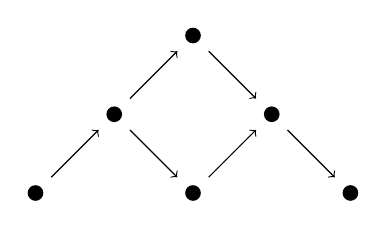
\begin{tikzpicture}
 		\node[circle,fill,inner sep=2pt] (a) at (0,0) {};
 		\node[circle,fill,inner sep=2pt] (b) at (1,1) {};
 		\node[circle,fill,inner sep=2pt] (c) at (2,0) {};
 		\node[circle,fill,inner sep=2pt] (d) at (2,2) {};
 		\node[circle,fill,inner sep=2pt] (e) at (3,1) {};
 		\node[circle,fill,inner sep=2pt] (f) at (4,0) {};

 		\draw[->,shorten <=5pt, shorten >=5pt] (a) -- (b);
 		\draw[->,shorten <=5pt, shorten >=5pt] (b) -- (c);
 		\draw[->,shorten <=5pt, shorten >=5pt] (b) -- (d);
 		\draw[->,shorten <=5pt, shorten >=5pt] (c) -- (e);
 		\draw[->,shorten <=5pt, shorten >=5pt] (d) -- (e);
 		\draw[->,shorten <=5pt, shorten >=5pt] (e) -- (f);
 	 \end{tikzpicture}
 \end{figure}
\end{frame}

\section{Higher Auslander Algebras \\ \normalsize
\textcolor{black!60!bgcolorAlt}{Cluster Tilting Modules, Cyclic Polytopes}}

\begin{frame}[fragile]
 \frametitle{Module extensions}
 \begin{alertblock}{The group of extensions}
 	An \alert{extension} of a $\Lambda$-module $M$ by a $\Lambda$-module $N$ is a
 	\alert{short exact sequence}
 	\begin{figure}[h]
 	 \centering
 	 \begin{tikzcd}
 	  0 \ar[r] & M \ar[r] & X \ar[r] & N \ar[r] & 0.
 	 \end{tikzcd}
 	\end{figure}
 	All the (equivalence classes of) extensions of $M$ by $N$ form a group which
 	we denote $\mathrm{Ext^{1}}(M,N)$.
 \end{alertblock}
 \pause
 This construction can be extended to `$n$-fold' extensions of $M$ by $N$, that
 is, \alert{long exact sequences}
 \begin{figure}[h]
  \centering
  \begin{tikzcd}
   0 \ar[r] & M \ar[r] & X_n \ar[r] & X_{n-1} \ar[r] & \cdots \ar[r] & X_1
   \ar[r] & N \ar[r] & 0.
  \end{tikzcd}
 \end{figure}
 The group of $n$-fold extensions of $M$ by $N$ is denoted
 $\mathrm{Ext}^{n}(M,N)$.
\end{frame}

\begin{frame}
 \frametitle{Cluster tilting modules}
 \begin{block}{$\add M$}
 	For a $\Lambda$-module $M$, we denote by $\add M$ the full subcategory of
 	$\cmod \Lambda$ whose objects are the direct sums of direct summands of $M$.
 \end{block}
 \pause
 \begin{alertblock}{$d$-cluster tilting module}
 	A $\Lambda$-module $M$ is $d$-cluster tilting if
 	\[
 	 \add M = \{X \in \cmod \Lambda \mid \mathrm{Ext}^{i}(X,M) = 0 \; \forall i
 	 \in \{1,\ldots,d-1\}\}.
 	\]
 \end{alertblock}
\end{frame}

\begin{frame}
 \frametitle{Higher Auslander algebras}
 \begin{const}[due to Iyama O.]
 	Let $\Lambda$ be a representation-finite hereditary algebra. Then, $\Lambda$
 	has a $1$-cluster tilting module $M^{(1)}$. Put $\Lambda^{(1)} \coloneqq
 	\mathrm{End}(M^{(1)})$.
 	\pause

 	The $k$-algebra $\Lambda^{(1)}$ has a $2$-cluster tilting module $M^{(2)}$.
 	Put $\Lambda^{(2)} \coloneqq \mathrm{End}(M^{(2)})$.
 	\pause

 	\centerline{$\vdots$}

 	The $k$-algebra $\Lambda^{(d)}$ has a $d$-cluster tilting module $M^{(d)}$.
 	Put $\Lambda^{(d+1)} \coloneqq \mathrm{End}(M^{(d)})$.
 \end{const}
 \pause
 The $k$-algebra $\Lambda^{(d)}$ is called the $d$-Auslander algebra of
 $\Lambda$.
\end{frame}

\begin{frame}[fragile]
 \frametitle{Higher Auslander algebras of type $A$}
 We apply Iyama's construction to $\Lambda \coloneqq k(\tikz[baseline=-3pt]{
 	\node[circle,fill,inner sep=1.5pt] (a) at (0,0) {};
 	\node[circle,fill,inner sep=1.5pt] (b) at (0.75,0) {};
 	\node[circle,fill,inner sep=1.5pt] (c) at (1.5,0) {};

 	\draw[<-,shorten <=2pt, shorten >=2pt] (a) -- (b);
 	\draw[<-,shorten <=2pt, shorten >=2pt] (b) -- (c);
 })$. The AR quivers of $\Lambda, \Lambda^{(1)}$ and $\Lambda^{(2)}$ are the
 following.
 \pause
 \begin{figure}[h]
  \centering
  \begin{subfigure}[t]{.49\textwidth}
   \centering
 	 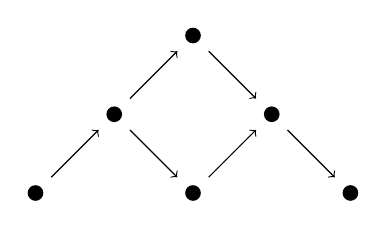
\begin{tikzpicture}
 		\node[circle,fill,inner sep=2pt] (a) at (0,0) {};
 		\node[circle,fill,inner sep=2pt] (b) at (1,1) {};
 		\node[circle,fill,inner sep=2pt] (c) at (2,0) {};
 		\node[circle,fill,inner sep=2pt] (d) at (2,2) {};
 		\node[circle,fill,inner sep=2pt] (e) at (3,1) {};
 		\node[circle,fill,inner sep=2pt] (f) at (4,0) {};

 		\draw[->,shorten <=5pt, shorten >=5pt] (a) -- (b);
 		\draw[->,shorten <=5pt, shorten >=5pt] (b) -- (c);
 		\draw[->,shorten <=5pt, shorten >=5pt] (b) -- (d);
 		\draw[->,shorten <=5pt, shorten >=5pt] (c) -- (e);
 		\draw[->,shorten <=5pt, shorten >=5pt] (d) -- (e);
 		\draw[->,shorten <=5pt, shorten >=5pt] (e) -- (f);
 	 \end{tikzpicture}
 	 \caption*{The AR quiver of $\Lambda$.}
  \end{subfigure}
  \pause
  \begin{subfigure}[t]{.49\textwidth}
   \centering
 	 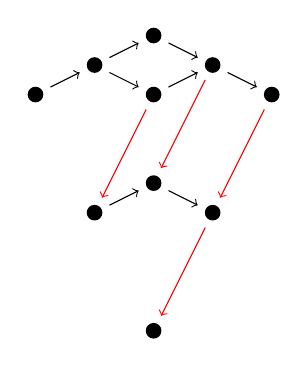
\begin{tikzpicture}[scale=0.75]
 		\node[circle,fill,inner sep=2pt] (a1) at (0,0) {};
 		\node[circle,fill,inner sep=2pt] (b1) at (1,0.5) {};
 		\node[circle,fill,inner sep=2pt] (c1) at (2,0) {};
 		\node[circle,fill,inner sep=2pt] (d1) at (2,1) {};
 		\node[circle,fill,inner sep=2pt] (e1) at (3,0.5) {};
 		\node[circle,fill,inner sep=2pt] (f1) at (4,0) {};

 		\draw[->,shorten <=3pt, shorten >=3pt] (a1) -- (b1);
 		\draw[->,shorten <=3pt, shorten >=3pt] (b1) -- (c1);
 		\draw[->,shorten <=3pt, shorten >=3pt] (b1) -- (d1);
 		\draw[->,shorten <=3pt, shorten >=3pt] (c1) -- (e1);
 		\draw[->,shorten <=3pt, shorten >=3pt] (d1) -- (e1);
 		\draw[->,shorten <=3pt, shorten >=3pt] (e1) -- (f1);

 		\node[circle,fill,inner sep=2pt] (c2) at (1,-2) {};
 		\node[circle,fill,inner sep=2pt] (e2) at (2,-1.5) {};
 		\node[circle,fill,inner sep=2pt] (f2) at (3,-2) {};

 		\draw[->,shorten <=3pt, shorten >=3pt] (c2) -- (e2);
 		\draw[->,shorten <=3pt, shorten >=3pt] (e2) -- (f2);

 		\draw[red,->,shorten <=3pt, shorten >=3pt] (c1) -- (c2);
 		\draw[red,->,shorten <=3pt, shorten >=3pt] (e1) -- (e2);
 		\draw[red,->,shorten <=3pt, shorten >=3pt] (f1) -- (f2);

 		\node[circle,fill,inner sep=2pt] (f3) at (2,-4) {};
 		\draw[red,->,shorten <=3pt, shorten >=3pt] (f2) -- (f3);
 	 \end{tikzpicture}
 	 \caption*{The AR quiver of $\Lambda^{(1)}$.}
  \end{subfigure}
 \end{figure}
\end{frame}

\begin{frame}[fragile]
 \frametitle{Higher Auslander algebras of type $A$}
 \begin{figure}[h]
  \centering
 	 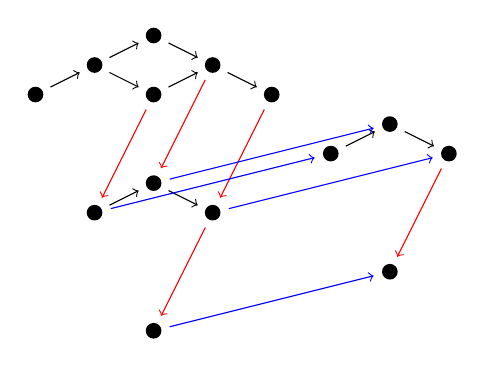
\begin{tikzpicture}[scale=0.75]
 		\node[circle,fill,inner sep=2pt] (a1) at (0,0) {};
 		\node[circle,fill,inner sep=2pt] (b1) at (1,0.5) {};
 		\node[circle,fill,inner sep=2pt] (c1) at (2,0) {};
 		\node[circle,fill,inner sep=2pt] (d1) at (2,1) {};
 		\node[circle,fill,inner sep=2pt] (e1) at (3,0.5) {};
 		\node[circle,fill,inner sep=2pt] (f1) at (4,0) {};

 		\draw[->,shorten <=3pt, shorten >=3pt] (a1) -- (b1);
 		\draw[->,shorten <=3pt, shorten >=3pt] (b1) -- (c1);
 		\draw[->,shorten <=3pt, shorten >=3pt] (b1) -- (d1);
 		\draw[->,shorten <=3pt, shorten >=3pt] (c1) -- (e1);
 		\draw[->,shorten <=3pt, shorten >=3pt] (d1) -- (e1);
 		\draw[->,shorten <=3pt, shorten >=3pt] (e1) -- (f1);

 		\node[circle,fill,inner sep=2pt] (c2) at (1,-2) {};
 		\node[circle,fill,inner sep=2pt] (e2) at (2,-1.5) {};
 		\node[circle,fill,inner sep=2pt] (f2) at (3,-2) {};

 		\draw[->,shorten <=3pt, shorten >=3pt] (c2) -- (e2);
 		\draw[->,shorten <=3pt, shorten >=3pt] (e2) -- (f2);

 		\draw[red,->,shorten <=3pt, shorten >=3pt] (c1) -- (c2);
 		\draw[red,->,shorten <=3pt, shorten >=3pt] (e1) -- (e2);
 		\draw[red,->,shorten <=3pt, shorten >=3pt] (f1) -- (f2);

 		\node[circle,fill,inner sep=2pt] (f3) at (2,-4) {};
 		\draw[red,->,shorten <=3pt, shorten >=3pt] (f2) -- (f3);

 		\node[circle,fill,inner sep=2pt] (c4) at (5,-1) {};
 		\node[circle,fill,inner sep=2pt] (e4) at (6,-0.5) {};
 		\node[circle,fill,inner sep=2pt] (f4) at (7,-1) {};

 		\draw[->,shorten <=3pt, shorten >=3pt] (c4) -- (e4);
 		\draw[->,shorten <=3pt, shorten >=3pt] (e4) -- (f4);

 		\node[circle,fill,inner sep=2pt] (f5) at (6,-3) {};
 		\draw[red,->,shorten <=3pt, shorten >=3pt] (f4) -- (f5);

 		\draw[blue,->,shorten <=3pt, shorten >=3pt] (c2) -- (c4);
 		\draw[blue,->,shorten <=3pt, shorten >=3pt] (e2) -- (e4);
 		\draw[blue,->,shorten <=3pt, shorten >=3pt] (f2) -- (f4);
 		\draw[blue,->,shorten <=3pt, shorten >=3pt] (f3) -- (f5);
 	 \end{tikzpicture}
  \caption*{The AR quiver of $\Lambda^{(2)}$.}
 \end{figure}
\end{frame}

\begin{frame}
 \frametitle{Cyclic polytopes}
 \begin{alertblock}{Cyclic polytope}
  The \alert{moment curve} is the map $p(t) = (t,t^2,t^3,\ldots,t^{n}) \subseteq
  \R^{n}$ for $t \in \R$. A \alert{cyclic polytope} $C(m,n)$ in $\R^{n}$ is the
  convex hull of the set $\{p(t_1),\ldots,p(t_m)\}$ where $t_1<t_2<\ldots<t_m$.
 \end{alertblock}
 \pause
 \textbf{Example.} The moment curve in $\R^2$ is just a parabola and $C(4,2)$ is
 the following shape (for $t_i = i - 1$).
 \begin{figure}[h]
  \centering
  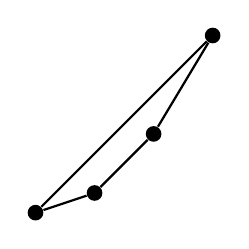
\begin{tikzpicture}[yscale=0.25,xscale=0.75]
   \node[circle,fill,inner sep=2pt] (a) at (0,0) {};
   \node[circle,fill,inner sep=2pt] (b) at (1,1) {};
   \node[circle,fill,inner sep=2pt] (c) at (2,4) {};
   \node[circle,fill,inner sep=2pt] (d) at (3,9) {};

   \draw[thick] (a) -- (b);
   \draw[thick] (b) -- (c);
   \draw[thick] (c) -- (d);
   \draw[thick] (d) -- (a);
  \end{tikzpicture}
 \end{figure}
\end{frame}

\begin{frame}
 \frametitle{Triangulations and tilting modules}
 \begin{alertblock}{A triangulation of a cyclic polytope}
  By a \alert{triangulation} of $C(m,n)$ we mean its division into
  $n$-dimensional simplices that share vertices with $C(m,n)$.
 \end{alertblock}
 \pause
 \textbf{Example}. One possible triangulation of $C(5,2)$.
 \begin{figure}[h]
  \centering
  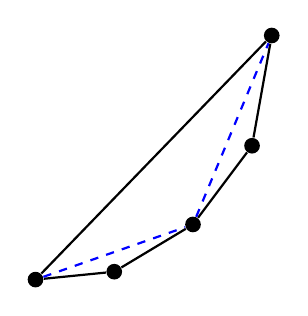
\begin{tikzpicture}[yscale=0.2,xscale=1]
   \node[circle,fill,inner sep=2pt] (a) at (0,0.5) {};
   \node[circle,fill,inner sep=2pt] (b) at (1,1) {};
   \node[circle,fill,inner sep=2pt] (c) at (2,4) {};
   \node[circle,fill,inner sep=2pt] (d) at (2.75,9) {};
   \node[circle,fill,inner sep=2pt] (e) at (3,16) {};

   \draw[thick] (a) -- (b);
   \draw[thick] (b) -- (c);
   \draw[thick] (c) -- (d);
   \draw[thick] (d) -- (e);
   \draw[thick] (e) -- (a);
   \draw[thick,blue,dashed] (a) -- (c);
   \draw[thick,blue,dashed] (c) -- (e);
  \end{tikzpicture}
 \end{figure}
\end{frame}

\begin{frame}[fragile]
 \frametitle{Triangulations and tilting modules}
 \begin{theorem}[Thomas H., Oppermann S.]
  There are bijections
  \begin{figure}[h]
   \centering
   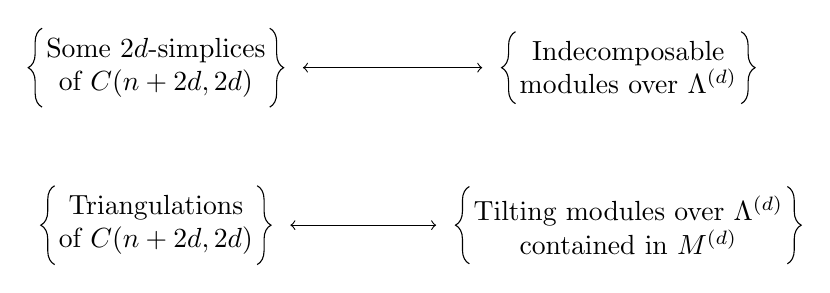
\begin{tikzpicture}
    \node[align=center] (a) at (0,0) {Some $2d$-simplices \\ of $C(n+2d,2d)$};
    \draw[decoration={brace,raise=-2pt,amplitude=5pt},decorate] (a.south west) --
     (a.north west);
    \draw[decoration={brace,mirror,raise=-2pt,amplitude=5pt},decorate] (a.south
     east) -- (a.north east);

    \node[align=center] (b) at (6,0) {Indecomposable \\ modules over
     $\Lambda^{(d)}$};
    \draw[decoration={brace,raise=-2pt,amplitude=5pt},decorate] (b.south west) --
     (b.north west);
    \draw[decoration={brace,mirror,raise=-2pt,amplitude=5pt},decorate] (b.south
     east) -- (b.north east);
    
    \draw[<->,shorten <=10pt, shorten >=10pt] (a.east) -- (b.west);
    
    \pause
    \begin{scope}[yshift=-2cm]
     \node[align=center] (a) at (0,0) {Triangulations \\ of $C(n + 2d,2d)$};
     \draw[decoration={brace,raise=-2pt,amplitude=5pt},decorate] (a.south west) --
      (a.north west);
     \draw[decoration={brace,mirror,raise=-2pt,amplitude=5pt},decorate] (a.south
      east) -- (a.north east);

     \node[align=center] (b) at (6,0) {Tilting modules over $\Lambda^{(d)}$ \\
      contained in $\add M^{(d)}$};
     \draw[decoration={brace,raise=-2pt,amplitude=5pt},decorate] (b.south west) --
      (b.north west);
     \draw[decoration={brace,mirror,raise=-2pt,amplitude=5pt},decorate] (b.south
      east) -- (b.north east);
     
     \draw[<->,shorten <=10pt, shorten >=10pt] (a.east) -- (b.west);
    \end{scope}
   \end{tikzpicture}
  \end{figure}
 \end{theorem}
\end{frame}
